\begin{figure}
    \caption{Estimated Counterfactual Values}
    \label{fig:ctrfct}
    \begin{subfigure}{\textwidth}
		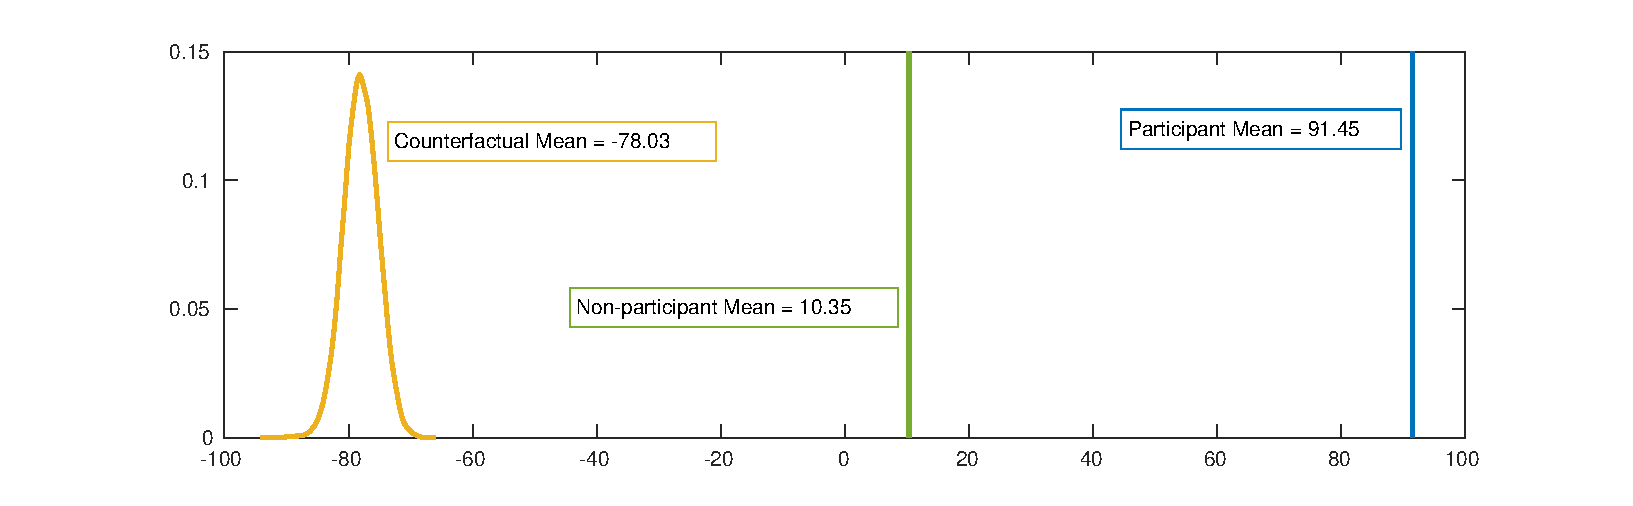
\includegraphics[scale=0.5]{./charts/counterfactual_cigwth_tech.eps}
		\caption{C\&I Loan Growth}
		\label{cigwth_c}
     \end{subfigure}
    %  \vfill
%      \begin{subfigure}{\textwidth}
%          %\begin{center}
% 		\includegraphics[scale=0.5]{./charts/counterfactual_cigwth_noppp_tech.eps}
% 		 %\end{center}
% 		 \caption{Non-PPP C\&I Loan Growth}
% 		 \label{cigwth_noppp_c}
%      \end{subfigure}
     \vfill
     \begin{subfigure}{\textwidth}
     %\begin{center}
		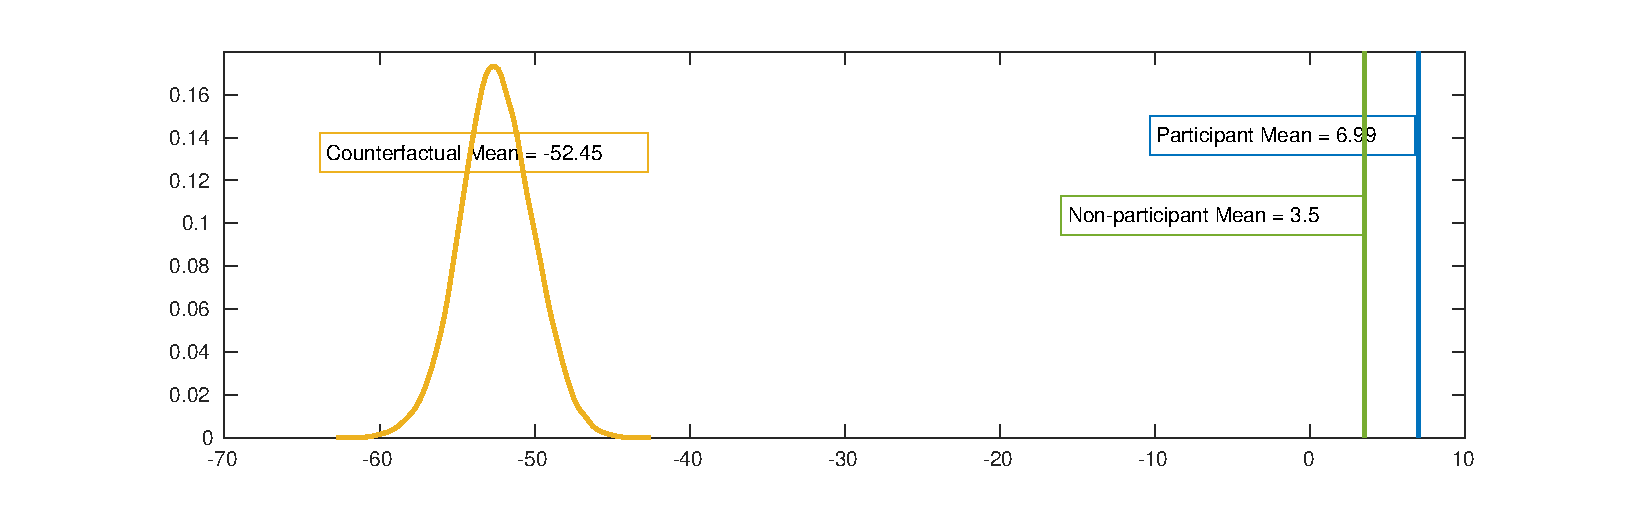
\includegraphics[scale=0.5]{./charts/counterfactual_cregwth_tech.eps}
			%\end{center}
		\caption{CRE Loan Growth}
		\label{cregwth_c}
     \end{subfigure}
     \vfill
     \begin{subfigure}{\textwidth}
      %\begin{center}
		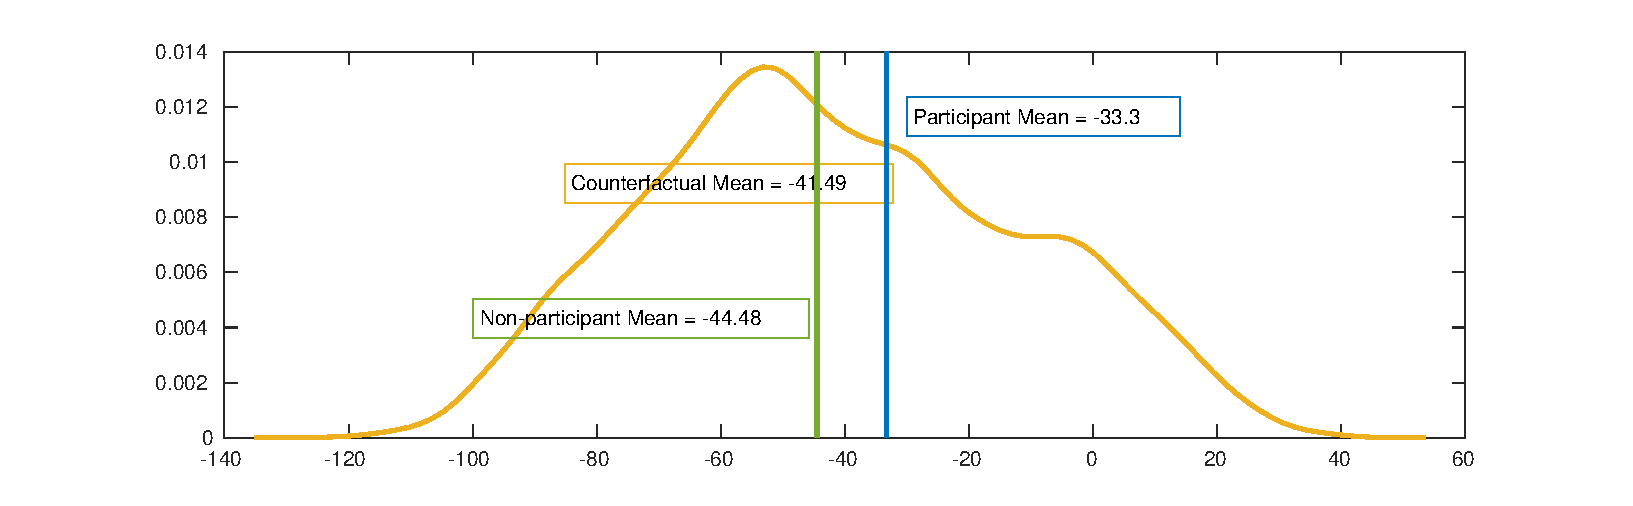
\includegraphics[scale=0.5]{./charts/counterfactual_dnim_tech.eps}
			%\end{center}
		 \caption{$\Delta$NIM}
		\label{nim_c}
     \end{subfigure}
     \\
\footnotesize Note: Charts show the posterior density of counterfactual average change in NIM for participating banks in the event of non-participation. The blue and green lines represent the realized average values for these categories for participants and non-participants, respectively, over year ending in Q2 and Q3 2020.
Source: Authors' calculations.
\end{figure}
